\section{Методы решения начальных и краевых задач для обыкновенных дифференциальных уравнений (ОДУ) и систем ОДУ}

\subsection{Постановка задачи}
4.1. Реализовать методы Эйлера, Рунге-Кутты и Адамса 4-го порядка в виде программ, задавая в качестве входных данных шаг сетки $h$. С использованием разработанного программного обеспечения решить задачу Коши для ОДУ 2-го порядка на указанном отрезке. Оценить погрешность численного решения с использованием метода Рунге – Ромберга и путем сравнения с точным решением. 

{\bfseries Вариант:} 20
    \begin{equation}
        x(x - 1)y'' + \frac{1}{2} y' - \frac{3}{4} y = 0\\
        y(2) = 2\sqrt{2}, \\
        y'(2) = \frac{3}{2} \sqrt{2}, \\
        x \in [2,3], h = 0.1
    \end{equation}
    
    \begin{equation}
		y = |x|^{3/2}
    \end{equation}
\pagebreak

\subsection{Результаты работы}
\begin{figure}[h!]
\centering
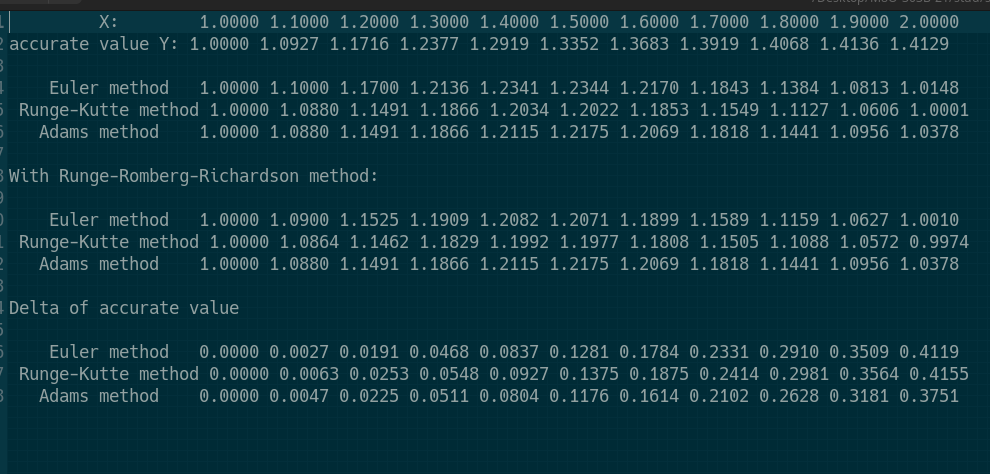
\includegraphics[width=.7\textwidth]{lab4.1}
\caption{Вывод в консоли}
\end{figure}


\subsection{Исходный код}
\lstinputlisting[title=\texttt{matrix.h}]{../stud/svoevolin/matrix.h}
\lstinputlisting[title=\texttt{4-1.cpp}]{../stud/svoevolin/4-1.cpp}
\pagebreak